\chapter{Theoretical Modeling and Robustness Analysis}

\label{Chapter-Theoretical-Modeling-and-Robustness-Analysis}

In this chapter, a model of CNNs structure, execution and characteristics is being created using MATLAB \cite{MATLAB-Official-site}. For a better understanding of the underlining algorithms, a C/C++ library was created to replicate PyTorch's \cite{PyTorch-Official-site} functionality, from image and parameter importing and formatting, to every CNN layer type needed for the network's inference. The library's results were evaluated using PyTorch's results. AlexNet \cite{ImageNet-classification-with-deep-convolutional-neural-networks} is used as a reference network for this analysis, with the parameters provided by the PyTorch's prebuilt and pre-trained model.

A Sensitivity Analysis was also performed to explore hardware implementation opportunities. Furthermore, various quantization techniques and algorithmic optimizations have been studied and tested to reduce memory footprint and better utilize hardware resources. Lastly, several implementation techniques and tools on the same functionality have been studied to minimize hardware resources and latency.

\section{PyTorch and C/C++ implementations}
Since PyTorch is a high abstraction framework, the recreation of its functionality to a lower abstraction level language, like C/C++, is a necessity for a complete understanding of the neural network's operation mechanism. Hence, after creating a C/C++ library capable of implementing most CNNs, it was evaluated for its correctness using PyTorch as a baseline. Its evaluation was conducted by implementing AlexNet as an example network, using both PyTorch and the C/C++ library, and then running the network's inference on both implementations. A subset of the ImageNet's database was used as input images, provided by Kaggle \cite{Kaggle}, which included 1250 images of cats and another 1250 images of dogs.

Afterward, the results, taken from the last FC layer of both implementations, were compared to create an error rate for each input. The library is designed in a way that it can use any data type for weights and activations to enable further experimentations. This evaluation experiment was conducted two times, one for using double-precision and another for using single-precision floating-point data type (IEEE standard). The error rate of both experiments was almost zero, with some minor inconsistencies between the floating-point representations of C/C++ and Python. Thus, both implementations' classifications were fully matched, and the library can be characterized as correct.

\subsection{Algorithms}
The main building blocks of a typical 2-D CNN are presented below. Every algorithm in this section is part of this work's aforementioned C/C++ library.

\subsubsection{Convolution}
Algorithm \ref{alg:Convolution-Layer} performs a 2-D Convolution on 3-D array inputs, like images. The \textit{input} is characterized by its height, its width, and its number of channels. In other words, the number of its parallel matrices; for an RGB image, there are three channels, one for every color. The \textit{kernelSize}, \textit{stride} and \textit{padding} are the hyper-parameters of convolution layers, and because they differ for every layer and network, they have to be included in the procedure's parameters. Last but not least, \textit{weights} and \textit{bias} are the networks parameters. This algorithm outputs a 3-D array with the convolution's results.

\begin{algorithm}[H]
	\caption{Convolution Layer}\label{alg:Convolution-Layer}
	\begin{algorithmic}[1]
		\Procedure{Convolution Layer}{input, kernelSize, stride, padding, weights, bias}
			\State $hOut \gets (input.height +2 * padding - kernelSize) / stride + 1$
			\State $wOut \gets (input.width +2 * padding - kernelSize) / stride + 1$

			\For{i:=1 \textbf{to} input.channels}
				\For{j:=1 \textbf{to} input.height + 2 * padding}
					\For{k:=1 \textbf{to} input.width + 2 * padding}
						\If{j <= padding || k <= padding || j > image.height + padding || k > image.width + padding}
							\State $arr(i, j, k) \gets 0$
						\Else{}
							\State $arr(i, j, k) \gets input(i, j - padding, k - padding)$
						\EndIf
					\EndFor
				\EndFor
			\EndFor

			\For{oc:=1 \textbf{to} size(weights, 1)} \Comment{\#Output channels}
				\For{oh:=1 \textbf{to} hOut}
					\State $imgStartH \gets oh * stride$
					\State $imgEndH \gets imgStartH + kernelSize$

					\For{ow:=1 \textbf{to} wOut}
						\State $imgStartW \gets ow * stride$
						\State $imgEndW \gets imgStartW + kernelSize$

						\State $pixel \gets 0$
						\For{ic:=1 \textbf{to} input.channels}
							\For{i:=1 \textbf{to} kernelSize}
								\For{j:=1 \textbf{to} kernelSize}
									\State $pixel \gets pixel + arr(ic, i + imgStartH, j + imgStartW) * weights(oc, ic, i, j)$
								\EndFor
							\EndFor
						\EndFor

						\State $output(oc, oh, ow) \gets pixel + bias(oc)$
					\EndFor
				\EndFor
			\EndFor
			\State \textbf{return} $output$
		\EndProcedure
	\end{algorithmic}
\end{algorithm}

Algorithm \ref{alg:Convolution-Layer-with-ReLU} is a slightly more optimized version of algorithm \ref{alg:Convolution-Layer}. Since padding creates areas of the input that are zeroed out, convolution on those areas results in zero. Therefore, the for-loops' indices are carefully calculated to avoid iterations on the padded areas. Furthermore, the creation of the "padded" input is also omitted.

Moreover, a small optimization is injecting the ReLU activation function into this algorithm. Provided that ReLU is used almost after every convolution layer, this optimization avoids rereading the whole input from memory to make a simple decision. The procedure's \textit{doRelu} parameter configures if the ReLU activation is used.

\begin{algorithm}[H]
	\caption{Convolution Layer with ReLU}\label{alg:Convolution-Layer-with-ReLU}
	\begin{algorithmic}[1]
		\Procedure{Convolution Layer with ReLU}{input, kernelSize, stride, padding, weights, bias, doRelu}
			\State $hOut \gets (input.height +2 * padding - kernelSize) / stride + 1$
			\State $wOut \gets (input.width +2 * padding - kernelSize) / stride + 1$

			\For{oc:=1 \textbf{to} size(weights, 1)} \Comment{\#Output channels}
				\For{oh:=1 \textbf{to} hOut}

					\State $imgStartH \gets oh * stride - padding$

					\State $iStart \gets imgStartH < 0 ? padding : 0$

					\If{$imgStartH + kernelSize \geq input.height$}
						\State $iEnd \gets kernelSize - (imgStartH + kernelSize - input.height)$
					\Else{}
						\State $iEnd \gets kernelSize$
					\EndIf

					\For{ow:=1 \textbf{to} wOut}
						\State $imgStartW \gets ow * stride - padding$

						\State $jStart \gets imgStartW < 0 ? padding : 0$

						\If{$imgStartW + kernelSize \geq input.height$}
							\State $jEnd \gets kernelSize - (imgStartW + kernelSize - input.height)$
						\Else{}
							\State $jEnd \gets kernelSize$
						\EndIf

						\State $pixel \gets bias(oc)$

						\For{ic:=1 \textbf{to} input.channels}
							\For{i:=iStart \textbf{to} iEnd}
								\For{j:=jStart \textbf{to} jEnd}
									\State $pixel \gets pixel + input(ic, i + imgStartH, j + imgStartW) * weights(oc, ic, i, j)$
								\EndFor
							\EndFor
						\EndFor

						\State $output(oc, oh, ow) \gets doRelu \&\& pixel < 0 ? 0 : pixel$
					\EndFor
				\EndFor
			\EndFor
			\State \textbf{return} $output$
		\EndProcedure
	\end{algorithmic}
\end{algorithm}

\subsubsection{MaxPool}
Algorithm \ref{alg:MaxPool-Layer} performs a 2-D max-pooling operation on 3-D array inputs. Likewise to the convolution algorithm's \textit{input}, it is characterized by its height, width, and channel number. Also the \textit{kernelSize} and \textit{stride} hyper-parameters are present, in contrast to padding, which is not used, so it is omitted. This algorithm outputs a 3-D array with the max-pooling operation's results.

\begin{algorithm}[H]
	\caption{MaxPool Layer}\label{alg:MaxPool-Layer}
	\begin{algorithmic}[1]
		\Procedure{MaxPool Layer}{input, kernelSize, stride}
			\State $hOut \gets (input.height - kernelSize) / stride + 1$
			\State $wOut \gets (input.width - kernelSize) / stride + 1$
			\For{i:=1 \textbf{to} input.channels}
				\For{j:=1 \textbf{to} hOut}
					\For{k:=1 \textbf{to} wOut}
						\State $max \gets -\infinity$
						\For{l:=1 \textbf{to} kernelSize}
							\For{m:=1 \textbf{to} kernelSize}
								\State $curHeight \gets j * stride + l$
								\State $curWidth \gets k * stride + l$
								\State $curPixel \gets input(i, curHeight, curWidth)$
								\If{max < curPixel}
									\State $max \gets curPixel$
								\EndIf
							\EndFor
						\EndFor
						\State $output(i, j, k) \gets max$
					\EndFor
				\EndFor
			\EndFor
			\State \textbf{return} $output$
		\EndProcedure
	\end{algorithmic}
\end{algorithm}

\subsubsection{Fully-Connected}
Algorithm \ref{alg:Fully-Connected-Layer} performs a matrix multiplication on the \textit{input} and \textit{weights}. The \textit{input} is a vector, either coming from the previous FC layer's output or the flattening of the previous convolution or max-pooling layer's results. After the matrix multiplication a \textit{bias} is accumulated. This algorithm outputs a vector with the results of the matrix multiplication.

\begin{algorithm}[H]
	\caption{Fully-Connected Layer}\label{alg:Fully-Connected-Layer}
	\begin{algorithmic}[1]
		\Procedure{Fully-Connected Layer}{input, weights, bias}
			\State $inputSize \gets size(input)$
			\State $outputSize \gets size(weights, 1)$
			\For{i:=1 \textbf{to} outputSize}
				\State $output(i)\gets bias(i)$
				\For{j:=1 \textbf{to} inputSize}
					\State $output(i)\gets output(i) + input(j) * weights(i, j)$
				\EndFor
				\If{doRelu \&\& output(i) < 0}
					\State $output(i) \gets 0$
				\EndIf
			\EndFor
			\State \textbf{return} $output$
		\EndProcedure
	\end{algorithmic}
\end{algorithm}

Algorithm \ref{alg:Fully-Connected-Layer-with-ReLU} is a slightly more optimized version of algorithm \ref{alg:Fully-Connected-Layer}. Likewise to the convolution algorithm \ref{alg:Convolution-Layer-with-ReLU}, the ReLU activation is injected and can be configured through the \textit{doReLU} parameter.

\begin{algorithm}[H]
	\caption{Fully-Connected Layer with ReLU}\label{alg:Fully-Connected-Layer-with-ReLU}
	\begin{algorithmic}[1]
		\Procedure{Fully-Connected Layer with ReLU}{input, weights, bias, doReLU}
			\State $inputSize \gets size(input)$
			\State $outputSize \gets size(weights, 1)$
			\For{i:=1 \textbf{to} outputSize}
				\State $output(i)\gets bias(i)$
				\For{j:=1 \textbf{to} inputSize}
					\State $output(i)\gets output(i) + input(j) * weights(i, j)$
				\EndFor
				\If{doRelu \&\& output(i) < 0}
					\State $output(i) \gets 0$
				\EndIf
			\EndFor
			\State \textbf{return} $output$
		\EndProcedure
	\end{algorithmic}
\end{algorithm}

\subsubsection{ReLU}
While ReLU activation function is already injected to the convolution \ref{alg:Convolution-Layer-with-ReLU} and FC \ref{alg:Fully-Connected-Layer-with-ReLU} algorithms, its algorithms are shown below for completeness. Algorithm \ref{alg:ReLU1D)} performs the ReLU activation on vector inputs, suitable for use after FC layers. Algorithm \ref{alg:ReLU3D)} performs the ReLU activation on 3-D data inputs, suitable for use after convolution and max pooling layers.

\begin{algorithm}[H]
	\caption{ReLU (1-D)}\label{alg:ReLU1D)}
	\begin{algorithmic}[1]
		\Procedure{ReLU (1-D)}{input}
			\For{i:=1 \textbf{to} size(input)}
				\If{input(i) > 0}
					\State $output(i) \gets input(i)$
				\Else{}
					\State $output(i) \gets 0$
				\EndIf
			\EndFor
			\State \textbf{return} $output$
		\EndProcedure
	\end{algorithmic}
\end{algorithm}

\begin{algorithm}[H]
	\caption{ReLU (3-D)}\label{alg:ReLU3D)}
	\begin{algorithmic}[1]
		\Procedure{ReLU (3-D)}{input}
			\For{i:=1 \textbf{to} size(input, 1)}
				\For{j:=1 \textbf{to} size(input, 2)}
					\For{k:=1 \textbf{to} size(input, 3)}
						\If{input(i, j, k) > 0}
							\State $output(i, j, k) \gets input(i, j, k)$
						\Else{}
							\State $output(i, j, k) \gets 0$
						\EndIf
					\EndFor
				\EndFor
			\EndFor
			\State \textbf{return} $output$
		\EndProcedure
	\end{algorithmic}
\end{algorithm}

\subsubsection{SoftMax}
Algorithm \ref{alg:SoftMax} performs a SoftMax activation function on vector inputs. This operation is applied after the last FC layer and outputs the probability distribution of each target class.

\begin{algorithm}[H]
	\caption{SoftMax}\label{alg:SoftMax}
	\begin{algorithmic}[1]
		\Procedure{SoftMax}{$input$}
			\State $sum \gets 0$

			\For{i:=1 \textbf{to} size(input)}
				\State $sum \gets sum + e^{input(i)}$
			\EndFor

			\For{i:=1 \textbf{to} size(input)}
				\State $output \gets e^{input(i)} / sum$
			\EndFor

			\State \textbf{return} $output$
		\EndProcedure
	\end{algorithmic}
\end{algorithm}

\section{Memory Footprint}
\label{sec:Memory-Footprint}
Memory footprint plays a considerable role in neural network applications based on FPGA or ASIC systems. While neural networks are compute-bound on classic hardware architectures, on FPGAs' and ASICs', they can become memory bound due to their high parallelism capabilities but low memory bandwidth. In general, an application can fully benefit from an FPGA when its memory requirements fit into the FPGA's internal BRAM. Otherwise, modern FPGAs support external DRAM modules that can be utilized to fulfill the application's memory requirements. However, this introduces latency and memory I/O stalls to the system.

Consequently, it is of high importance to minimize the network's memory footprint in order to make it fit into the internal BRAM, or at least, minimize the memory bandwidth requirements. It is firstly needed to explore how the network's memory requirements are distributed throughout its stages. Using AlexNet as a reference network, tables \ref{tab:AlexNet-Parameters-Memory-Footprint} and \ref{tab:AlexNet-Data-Stages-Memory-Footprint} show AlexNet's parameters memory requirements per layer and each layer's output memory requirements respectively, using single-precision floating-point numbers.

\begin{table}[H]
	\caption{AlexNet Parameters Memory Footprint}
	\label{tab:AlexNet-Parameters-Memory-Footprint}
	\centering
	\begin{tabular}{llll}
		\toprule
		\textbf{Layer} & \textbf{\#Parameters} & \textbf{Footprint} & \textbf{Memory (\%)}  \\
		\midrule
			Conv1 & $64 * 3 * 11 * 11 = 23232$ & 92.92KB & 0.04 \\
			Conv2 & $192 * 64 * 5 * 5 = 307200$ & 1.22MB & 0.5 \\
			Conv3 & $384 * 192 * 3 * 3 = 663552$ & 2.65MB & 1.09 \\
			Conv4 & $256 * 384 * 3 * 3 = 884736$ & 3.53MB & 1.45 \\
			Conv5 & $256 * 256 * 3 * 3 = 589824$ & 2.35MB & 0.97 \\
			FC1 & $9216 * 4096 = 37748736$ & 150.99MB & 61.79 \\
			FC2 & $4096 * 4096 = 16777216$ & 67.10MB & 27.46 \\
			FC3 & $4096 * 1000 = 4096000$ & 16.38MB & 6.70 \\
		\midrule
			\textbf{Total} & 61090496 & 244.36MB & 100 \\
		\bottomrule
	\end{tabular}
\end{table}

This work focuses on the Xilinx ZCU102 \cite{ZCU102-User-Guide} \cite{ZCU102-Product-Overview} and the QFDB \cite{Implementation-and-Impact-of-an-Ultra-Compact-Multi-FPGA-Board-for-Large-System-Prototyping} target boards, which both integrate the same Zynq UltraScale+ MPSoC XCZU9EG-2FFVB1156E (for more information see section \ref{sec:FPGA-Platforms}). Unfortunately, this MPSoC provides only 2MBs of BRAM, which, according to tables \ref{tab:AlexNet-Parameters-Memory-Footprint} and \ref{tab:AlexNet-Data-Stages-Memory-Footprint}, creates some serious memory constraints.

In respect to table \ref{tab:AlexNet-Parameters-Memory-Footprint}, only the first and the second convolutional layers' parameters can fit both simultaneously in the MPSoC's BRAM. Moreover, not only do all other layers not fit, but they also need up to 75 times more memory each (see first Fully-Connected layer).

\begin{table}[H]
	\caption{AlexNet Data Stages Memory Footprint.}
	\label{tab:AlexNet-Data-Stages-Memory-Footprint}
	\centering
	\begin{tabular}{llll}
		\toprule
		\textbf{Layer} & \textbf{\#Data} & \textbf{Footprint} & \textbf{Memory (\%)}  \\
		\midrule
			Image & $3 * 224 * 224 = 150528$ & 150.52KB & 6.07 \\
			Conv1 & $64 * 55 * 55 = 193600$ & 774.40KB & 31.22 \\
			MaxPool1 & $64 * 27 * 27 = 46656$ & 186.62KB & 7.52 \\
			Conv2 & $192 * 27 * 27 = 139968$ & 559.87KB & 22.57 \\
			MaxPool2 & $192 * 13 * 13 = 32448$ & 129.79KB & 5.23 \\
			Conv3 & $384 * 13 * 13 = 64896$ & 259.58KB & 10.46 \\
			Conv4 & $256 * 13 * 13 = 43264$ & 173.05KB & 6.98 \\
			Conv5 & $256 * 13 * 13 = 43264$ & 173.05KB & 6.98 \\
			MaxPool3 & $9216$ & 36.86KB & 1.49 \\
			FC1 & $4096$ & 16.38KB & 0.66 \\
			FC2 & $4096$ & 16.38KB & 0.66 \\
			FC3 & $1000$ & 4KB & 0.16 \\
		\midrule
			\textbf{Total} & 682856 & 2.48MB & 100 \\
		\bottomrule
	\end{tabular}
\end{table}

In respect to table \ref{tab:AlexNet-Data-Stages-Memory-Footprint}, all layers' outputs can fit individually into the MPSoC's BRAM; however, they cannot fit all together combined.

Under those circumstances, the exploration of various techniques for memory footprint reduction, memory footprint partitioning, and caching is an essential requirement.

\section{Data Types}
As mentioned in the Related Work section, memory bandwidth needs can become a severe bottleneck to applications like neural networks on FPGAs and ASICs. Consequently, the investigation of the most suitable data type for parameters and activations is a necessity. However, decreasing the bit-width does come with its costs, classification accuracy. This creates a tradeoff between network classification accuracy and inference speed. In general, lowering the bit-width increases performance due to both decreasing memory bandwidth and computation time, but decreases accuracy. The cost of each bit-width lowering is different for every application, so an application-specific investigation has to be conducted.

\subsection{Evaluation}
Using AlexNet as a reference, various data types have been tested to achieve the best performance to accuracy ratio. From double, single, and half-precision floating-point (IEEE standard) representations to fixed-point from 64 down to 8-bit representations have been tested. This experiment's baseline uses a single-precision floating-point, as it is the pre-trained model's data type. After inferencing 2500 images using every data type, each image classification Top-1 result was compared to the baseline's result. The Top-1 error rates for each data type are presented in tables \ref{tab:floats-error-rates} and \ref{tab:fixed-error-rates}.

\subsection{Floating Point}
It is worth noting that a MATLAB implementation of the network had to be used in this investigation, due to the fact that, at the time of writing, neither PyTorch nor C/C++ support half-precision floating-point arithmetic. Unfortunately, MATLAB inference was really slow compared to PyTorch, and even slower when using half-precision (see table \ref{tab:floats-error-rates} Avg. inference time column). The half-precision floating-point slowdown was caused because there is no hardware acceleration on the test CPU (Intel i7 4710MQ \cite{Intel-i7-4710MQ-Processor}) for such data type, forcing the mathematical operations to be calculated using software emulation.

Before every test, the network's parameters were converted from the given single-precision floating-point pre-trained model to the corresponding data type. Also, the same data type was used for the layers' activations during inference. While converting single-precision to double-precision does not result in higher arithmetic accuracy, experiments with doubles were conducted for completeness, as shown in table \ref{tab:floats-error-rates}.

\begin{table}[H]
	\caption{Top-1 error rate of every floating-point tested data type.}
	\label{tab:floats-error-rates}
	\centering
	\begin{tabular}{p{2cm} p{2cm} p{3cm} p{3cm}}
		\toprule
		\textbf{Tool} & \textbf{Data type} & \textbf{Top-1 Error rate (\%)} & \textbf{Avg. inference time (sec)} \\
		\midrule
			PyTorch & float64	& 0			& 0.091 \\
			PyTorch & float32	& 0			& 0.034 \\
			MATLAB 	& float64	& 0			& 6.624 \\
			MATLAB 	& float32	& 0			& 8.162 \\
			MATLAB 	& float16 	& 0.36  	& 147.480 \\
		\bottomrule
	\end{tabular}
\end{table}

In respect to the floating-point data types, the Top-1 error-rate for both double and single-precision is zero, while for the half-precision, there is a minor error rate that can be ignored. As a result, the half-precision is the leading one in the floating-point space due to its excellent performance to accuracy ratio.

\subsection{Fixed Point}
\label{sec:fixed-point}
The usage of fixed-point data types can benefit the application with its lower memory bandwidth and its more straightforward hardware requirements and faster arithmetic operations compared to the floating-point data types. In contrast to the floating-point data types conversion, when converting to fixed-point data types, it is vital to select the position of the radix point that most accurately represents the given numbers. In this experiment, the uniform conversion technique was used in which given a set of numbers \emph{S} and the wanted representation bit width, \emph{W}, the radix point is selected as shown on equation \ref{eqn:select-radix-point-position} by minimizing the overall error between the given number set \emph{S} and the converted to fixed-point number set.
\begin{equation}
	\label{eqn:select-radix-point-position}
	Position = argmin_{i=0}^{W}[\frac{\sum_{j=1}^{size(S)} |S_j - FixPtConvert(S_j, W, i)| }{size(S)}]
\end{equation}
In this experiment, a different radix point position was calculated for every layer's parameters and every bit width with respect to each layer parameter's characteristics. This technique was first introduced by Williamson in 1991 \cite{Dynamically-scaled-fixed-point-arithmetic}, and is called Dynamic Fixed-Point arithmetic. Instead of using a global scaling factor for all layers (ordinary fixed-point arithmetic), dynamic fixed-point arithmetic uses a different scaling factor for every layer. On low bit-widths, using dynamic fixed-point because it can maintain most of the weights representation accuracy.

It should be mentioned that MATLAB's conversion of floating-point to any bit-width fixed-point data types results in a set of double-precision floating-point numbers to enable mathematical operations without needing fixed-point hardware acceleration or software emulation. Consequently, each layer's activations had to be converted to fixed-point so that the system's modeling was as accurate as possible.

Unfortunately, only the 64 and 32-bit tests resulted in no Top-1 error-rate, as shown in table \ref{tab:fixed-error-rates}. Even the 16-bit test resulted in a very high error-rate, rendering this data type unusable for this application. However, the high error-rate can be explained after visualizing the weights' distributions before and after the conversion, with its three side effects. The following figures were selected because of their dramatic transformation caused by this conversion to demonstrate its side effects.

\begin{table}[H]
	\caption{Top-1 error rate of every fixed-point tested data type.}
	\label{tab:fixed-error-rates}
	\centering
	\begin{tabular}{p{2cm} p{2cm} p{3cm} p{3cm}}
		\toprule
		\textbf{Tool} & \textbf{Data type} & \textbf{Top-1 Error rate (\%)} & \textbf{Avg. inference time (sec)} \\
			MATLAB 	& fixed64	& 0 		& 7.318 \\
			MATLAB 	& fixed32	& 0 		& 7.692 \\
			MATLAB 	& fixed16	& 22 		& 6.650 \\
			MATLAB 	& fixed14	& 28.44 	& 6.813 \\
			MATLAB 	& fixed12	& 36.24 	& 6.797 \\
			MATLAB 	& fixed10	& 77.07		& 6.929 \\
			MATLAB 	& fixed8	& 100 		& 6.312 \\
		\bottomrule
	\end{tabular}
\end{table}

First of all, figure \ref{fig:weight-distribution-comparison-conv2} depicts the second convolution layer's weights distributions of both their original single-precision floating-point and their 8-bit fixed-point converted representations. It is evident that the right histogram's limits have been significantly altered, with the weights $W \epsilon (-\infinity, -0.5) \cup (0.5, \infinity)$ been suppressed to the $(-0.5, 0.5)$ range.

\begin{figure} [H]
	\centering
	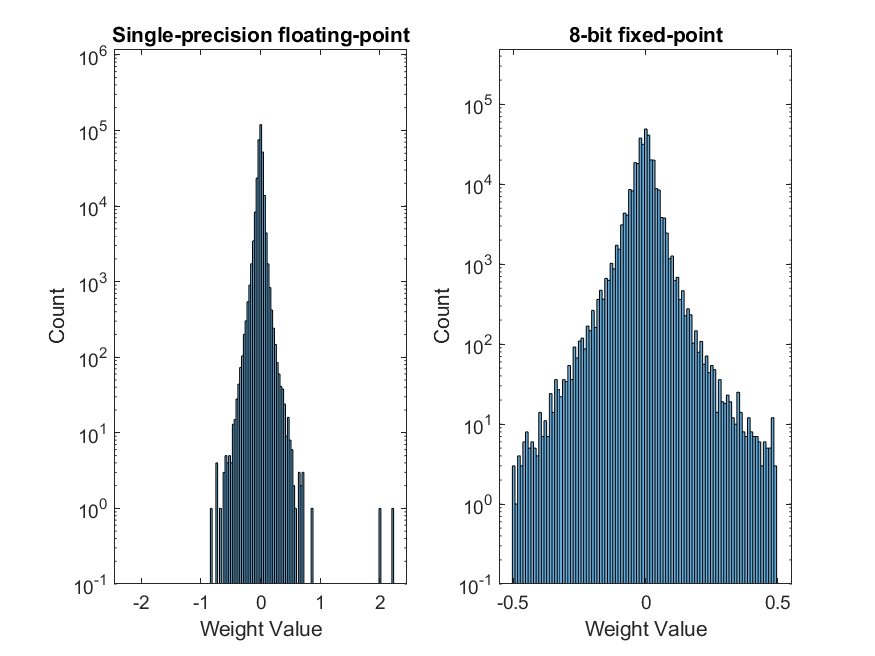
\includegraphics[scale=0.9]{../Images/Weights-distributions/original-vs-fixed8/weight-distribution-conv2.png}
	\decoRule
	\caption[Second Convolution layer's weights distribution comparison between single-precision floating-point and 8-bit fixed-point representations]{Second Convolution layer's weights distribution comparison between single-precision floating-point and 8-bit fixed-point representations: right histogram's limits are significantly altered.}
	\label{fig:weight-distribution-comparison-conv2}
\end{figure}

This suppression is caused by the nature of the 8-bit fixed-point data type, which only allows 256 different values to be represented. Equation's \ref{eqn:select-radix-point-position} result is position 8, which means that the representation's step is $1/2^8 = 0.00390625$, hence its limits are $-2^7/2^8 = -0.5$ and $2^7/2^8 = 0.5$ (the most significant bit is used for the sign). Although there are some weights in the range of $(-2, -0.5) \cup (0.5, 2)$, their summed conversion accuracy error is less than the sum of accuracy errors of the smaller numbers, which are orders of magnitude more in count, when another radix-point position is selected. In other words, the sum of a lot of small errors is greater than the sum of a few big errors, causing the big errors the be ignored.

Second of all, figure \ref{fig:weight-distribution-comparison-conv5} depicts the fifth convolution layer's weights distributions of both their original single-precision floating-point and their 8-bit fixed-point converted representations. While this layer's weights distribution limits are not altered, various spikes on the right histogram can be observed.

\begin{figure} [H]
	\centering
	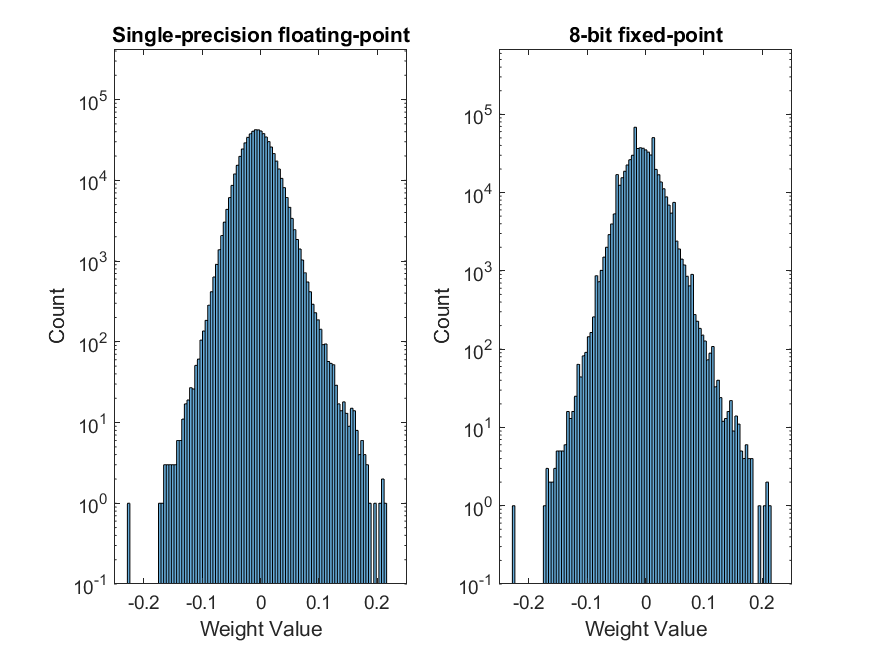
\includegraphics[scale=0.9]{../Images/Weights-distributions/original-vs-fixed8/weight-distribution-conv5.png}
	\decoRule
	\caption[Fifth Convolution layer's weights distribution comparison between single-precision floating-point and 8-bit fixed-point representations]{Fifth Convolution layer's weights distribution comparison between single-precision floating-point and 8-bit fixed-point representations: various spikes can be observed on the right histogram.}
	\label{fig:weight-distribution-comparison-conv5}
\end{figure}

Those spikes are caused by the fixed-point's inability to represent all real numbers. It is the same reason the floating-point data type exists. The fifth convolution layer's radix-point is positioned on the 8th bit, which results in a representation step of $1/2^8 = 0.00390625$. This means that any weight with value ($i/8, (i + 1)/8)$, with $i=-2^7, -2^7 + 1, ..., 2^7$, is rounded to the nearest fixed-point number available. Therefore, many weights are rounded to their nearest fixed-point representation, creating those spikes, which is expected.

Last but not least, figure \ref{fig:weight-distribution-comparison-FC1} depicts the first Fully-Connected layer's weights distributions of both their original single-precision floating-point and their 8-bit fixed-point converted representations. In this figure's right histogram, a high amount of subsampling can be observed compared to the left one.

\begin{figure} [H]
	\centering
	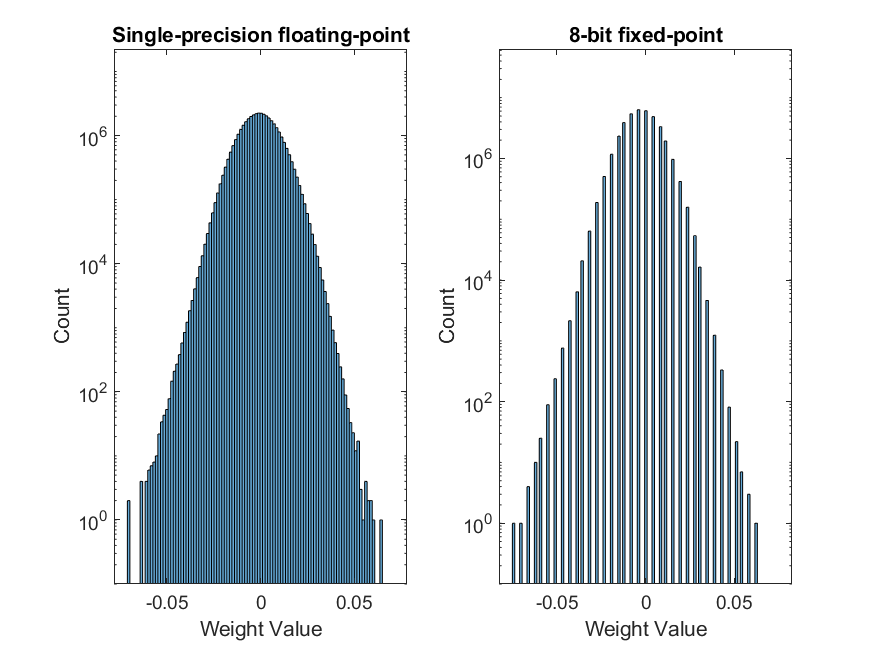
\includegraphics[scale=0.9]{../Images/Weights-distributions/original-vs-fixed8/weight-distribution-FC1.png}
	\decoRule
	\caption[First Fully-Connected layer's weights distribution comparison between single-precision floating-point and 8-bit fixed-point representations]{First Fully-Connected layer's weights distribution comparison between single-precision floating-point and 8-bit fixed-point representations: significant subsampling on the right histogram.}
	\label{fig:weight-distribution-comparison-FC1}
\end{figure}

Again, this subsampling can be explained by the fixed-point's inability to represent all weights accurately, resulting in jumps. In this layer, equation \ref{eqn:select-radix-point-position} positioned the radix-point on the 8th bit, which, again, means a step of $1/2^8 = 0.00390625$.

To tackle with the suppression and subsampling side effects, an enhanced version of this technique was used. More specifically, instead of merely measuring the representation error of each weight and the summing it up with all other errors, as equation \ref{eqn:select-radix-point-position} does, it is essential to further amplify significant errors in order for them to stand out compared to the big count of small errors. This amplification can be done by adding non-linearity to the error's computation. The Mean Squared Error (MSE) can be used for this purpose, as shown in equation \ref{eqn:select-radix-point-position-Mean-Squared-Error}.

After observing the weights' distributions, it is clear that some distributions need a more accurate representation step. This is given by the radix point's position. So, instead of searching for a position on the given bit width, the radix-point should be allowed to exceed the number's bit-width. Therefore, the maximum radix-point was selected greedily to be 32.

\begin{equation}
	\label{eqn:select-radix-point-position-Mean-Squared-Error}
	Position = argmin_{i=0}^{32}[\frac{\sum_{j=1}^{size(S)} |S_j - FixPtConvert(S_j, W, i)|^2 }{size(S)}]
\end{equation}

Although equation \ref{eqn:select-radix-point-position-Mean-Squared-Error} resulted in better inference accuracy, after some experimentation, more amplification was needed to achieve the best accuracy possible with this technique. For AlexNet, the Mean Quarted Error (MQE), shown on equation \ref{eqn:select-radix-point-position-Mean-Quarted-Error}, yields the best results, and no further amplification is needed.

\begin{equation}
	\label{eqn:select-radix-point-position-Mean-Quarted-Error}
	Position = argmin_{i=0}^{32}[\frac{\sum_{j=1}^{size(S)} |S_j - FixPtConvert(S_j, W, i)|^4 }{size(S)}]
\end{equation}

As shown on figures \ref{fig:weight-distribution-comparison-conv2-MQE}, \ref{fig:weight-distribution-comparison-conv5-MQE} and \ref{fig:weight-distribution-comparison-FC1-MQE}, the suppression and the subsampling side effects are eliminated. There is still some spiking; however, it is expected behavior due to the lack of representation accuracy with fixed-point data types.

\begin{figure} [H]
	\centering
	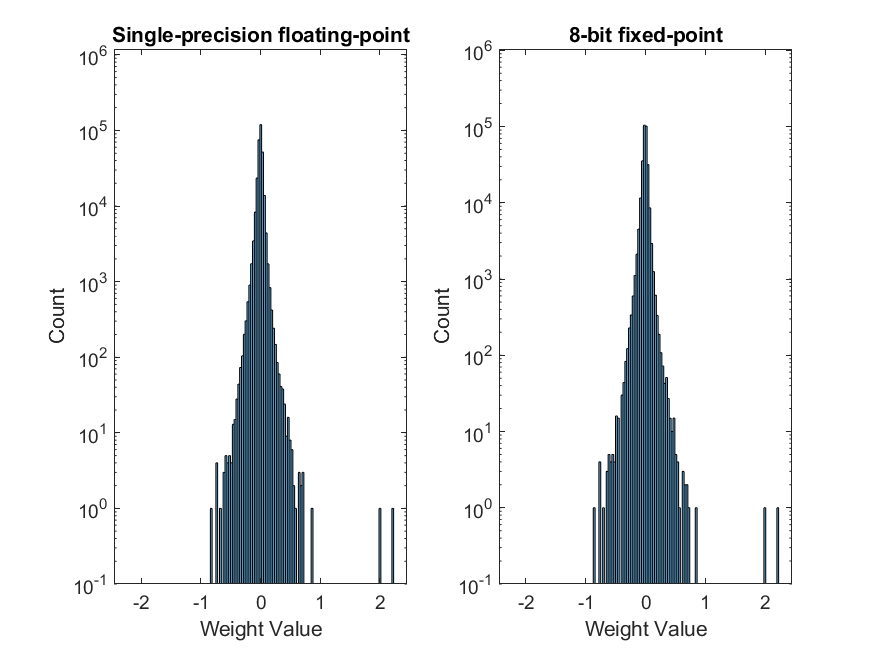
\includegraphics[scale=0.9]{../Images/Weights-distributions/original-vs-fixed8/weight-distribution-conv2-MQE.png}
	\decoRule
	\caption[Second Convolution layer's weights distribution comparison between single-precision floating-point and 8-bit fixed-point representations using MQE]{Second Convolution layer's weights distribution comparison between single-precision floating-point and 8-bit fixed-point representations using MQE: right histogram's limits are identical.}
	\label{fig:weight-distribution-comparison-conv2-MQE}
\end{figure}

Using MQE, equation \ref{eqn:select-radix-point-position-Mean-Quarted-Error} resulted in the 5th radix-point position for the second convolution layer's weights. This results in a representation step of $1/2^5 = 0.03125$, hence its limits are $-2^7/2^5 = -4$ and $2^7/2^5 = 4$. Consequently, the whole weights range can be represented, removing the suppression problem.

\begin{figure} [H]
	\centering
	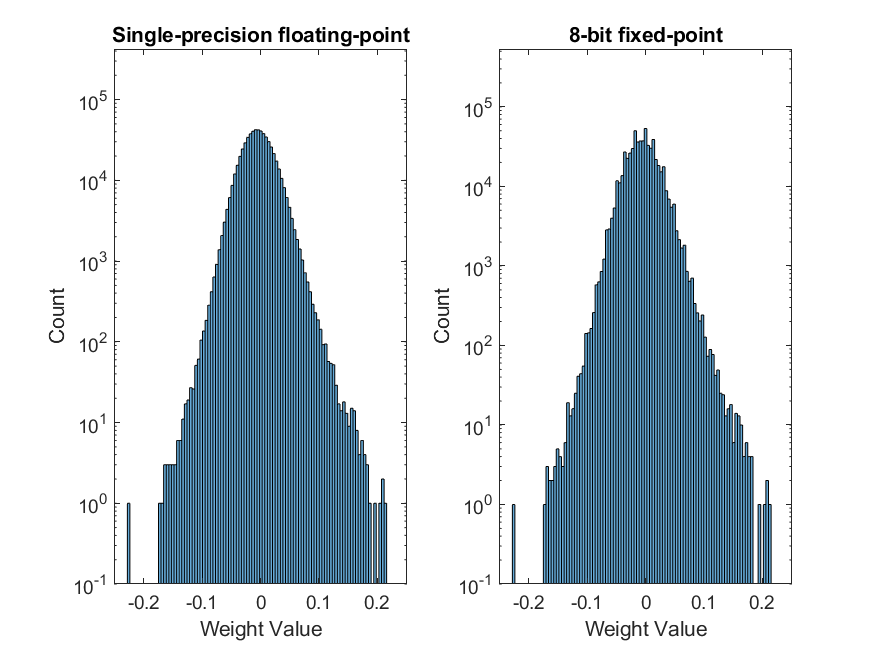
\includegraphics[scale=0.9]{../Images/Weights-distributions/original-vs-fixed8/weight-distribution-conv5-MQE.png}
	\decoRule
	\caption[Fifth Convolution layer's weights distribution comparison between single-precision floating-point and 8-bit fixed-point representations using MQE]{Fifth Convolution layer's weights distribution comparison between single-precision floating-point and 8-bit fixed-point representations using MQE: various spikes can still be observed on the right histogram.}
	\label{fig:weight-distribution-comparison-conv5-MQE}
\end{figure}

Using MQE, equation \ref{eqn:select-radix-point-position-Mean-Quarted-Error} resulted in the 9th radix-point position for the fifth convolution layer's weights. This results in a representation step of $1/2^9 = 0.001953125$, hence its limits are $-2^7/2^9 = -0.25$ and $2^7/2^9 = 0.25$. Although, the spikes are not removed, there is a slight improvement in the weights representation accuracy.

\begin{figure} [H]
	\centering
	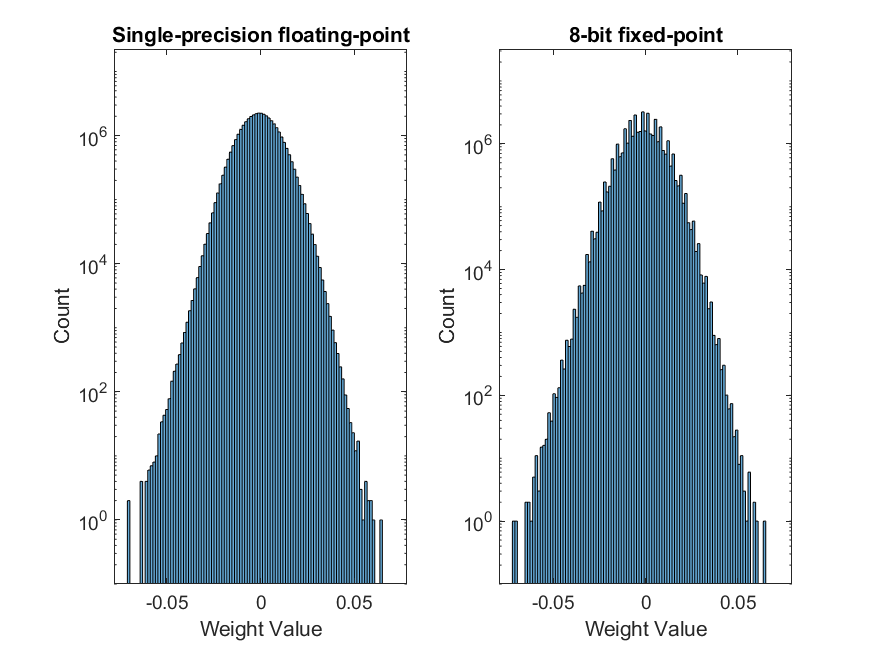
\includegraphics[scale=0.9]{../Images/Weights-distributions/original-vs-fixed8/weight-distribution-FC1-MQE.png}
	\decoRule
	\caption[First Fully-Connected layer's weights distribution comparison between single-precision floating-point and 8-bit fixed-point representations using MQE]{First Fully-Connected layer's weights distribution comparison between single-precision floating-point and 8-bit fixed-point representations using MQE: no subsampling on the right histogram.}
	\label{fig:weight-distribution-comparison-FC1-MQE}
\end{figure}

Using MQE, equation \ref{eqn:select-radix-point-position-Mean-Quarted-Error} resulted in the 10th radix-point position for the first Fully-Connected layer's weights. This results in a representation step of $1/2^10 = 0.0009765625$, hence its limits are $-2^7/2^10 = -0.125$ and $2^7/2^10 = 0.125$. The added representation accuracy fully eliminates the subsampling problem, though some spiking is introduced as expected.

Table \ref{tab:fixed-MQE-error-rates} shows the Top-1 error-rate of fixed-point data types using the Mean Quarted Error equation \ref{eqn:select-radix-point-position-Mean-Quarted-Error}. While 8, 10, and 12 bit width fixed-point data types are still unusable, the 14 and 16 bit width representations have improved significantly.

\begin{table}[H]
	\caption{Top-1 error rate of fixed-point data types using Mean Quarted Error equation \ref{eqn:select-radix-point-position-Mean-Quarted-Error}.}
	\label{tab:fixed-MQE-error-rates}
	\centering
	\begin{tabular}{lll}
		\toprule
		\textbf{Tool} & \textbf{Data type} & \textbf{Top-1 Error rate (\%)}\\
		\midrule
			MATLAB 	& fixed64	& 0 	\\
			MATLAB 	& fixed32	& 0 	\\
			MATLAB 	& fixed16	& 4.42 	\\
			MATLAB 	& fixed14	& 17.59 \\
			MATLAB 	& fixed12	& 48.11 \\
			MATLAB 	& fixed10	& 86.91	\\
			MATLAB 	& fixed8	& 99.3 	\\
		\bottomrule
	\end{tabular}
\end{table}

For better clarity on the results, figure \ref{fig:data-types-accuracy-chart} depicts all tested data types and their Top-1 accuracy.

\begin{figure} [H]
	\centering
	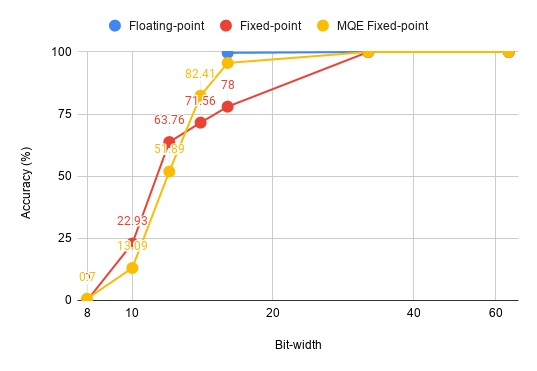
\includegraphics[width=\textwidth]{../Images/Weights-distributions/data-types-accuracy-chart.png}
	\decoRule
	\caption[All data types tested accuracy]{All data types tested accuracy.}
	\label{fig:data-types-accuracy-chart}
\end{figure}

After some experimentation, dynamically assigning different bit-widths on each layer, according to its accuracy needs, rather than a single bit-width for the whole network, can yield even better results. However, further investigation has to be conducted.

\subsection{Fixed Point Activations}
\label{sec:Fixed-Point-Activations}
Since floating-point arithmetic handles scaling automatically, the network does not face any overflow defects on its activations. However, when using fixed-point arithmetic, activations overflow is a severe problem. For instance, when multiplying 8-bit fixed point activations and weights, a new activation is generated with at most 16-bit width. Furthermore, adding two 16-bit activations can generate a new activation of 17-bit width. Therefore, if activations are not quantized between each layer, there will be a very wide output at the end of the network, wasting resources and performance when implemented in FPGAs.

Hence, between every layer, the activations should be quantized from their high-detail, large bit-width representations, back to some low bit wide representation. A question arises on how to quantize them in order to keep the most detail available. This work tries to keep the upper n bits from the first one. For example, let an activation implementation be 32-bit wide, its most significant one be on the 17th bit, and the new, low-detail representation be 8-bit wide. Then, if the upper 8 bits are kept, from the 31st bit down to the 24th bit, they will all be zeros, and as a result, its value will be lost. However, if the 8 bits from the first upper one are kept, from the 17th bit down to the 10th bit, the most significant detail is retained.

On the contrary, finding the most significant one on every activation in a single layer is not only computationally intensive but also requires that every activation has its own scale factor, rendering the fixed-point's benefits obsolete. All activations in a single layer should have the same scale factor, simplifying their arithmetic operations and minimizing required I/O.

Hence, an experiment was conducted to find each layer's optimal activation scale factor, whose results are depicted in table \ref{tab:Theoretical-and-Practical-activations-bit-widths}, using AlexNet as a reference. The theoretical bit-width represents the maximum bits needed to represent the layer's output adequately and can be calculated using equation \ref{eqn:theoretical-activation-bit-width}.
\begin{equation}
	\label{eqn:theoretical-activation-bit-width}
	Theoretical_{bitWidth} = input_{bitWidth} + weight_{bitWidth} + \lceil \log_2 \#Additions \rceil
\end{equation}

However, equation \ref{eqn:theoretical-activation-bit-width} calculates the maximum bit-width that could be generated after all operations, when all numbers are of max value, which is not the case. Therefore, the experiment includes a practical study of the maximum incurring bit-width, conducted by inferencing 2000 images and finding the maximum valued activation on each layer. Results of this experiment are depicted on column Practical bit-width of table \ref{tab:Theoretical-and-Practical-activations-bit-widths}.

\begin{table}[H]
	\caption{Theoretical and Practical activations' bit-widths}
	\label{tab:Theoretical-and-Practical-activations-bit-widths}
	\centering
	\begin{tabular}{lll}
		\toprule
		\textbf{Layer} & \textbf{Theoretical bit-width} & \textbf{Practical bit-width}\\
		\midrule
			Input & 8 & 8\\
			Conv1 & $ 8 + 8 + \lceil \log_2 3 * 11 * 11 \rceil = 25 $ & 17\\
			Conv2 & $ 8 + 8 + \lceil \log_2 64 * 5 * 5 \rceil = 27$ & 14\\
			Conv3 & $ 8 + 8 + \lceil \log_2 192 * 3 * 3 \rceil = 27$ & 15\\
			Conv4 & $ 8 + 8 + \lceil \log_2 384 * 3 * 3 \rceil = 28$ & 15\\
			Conv5 & $ 8 + 8 + \lceil \log_2 256 * 3 * 3 \rceil = 28$ & 17\\
			FC1 & $ 8 + 8 + \lceil \log_2 9216 \rceil = 30$ & 17\\
			FC2 & $ 8 + 8 + \lceil \log_2 4096 \rceil = 28$ & 17\\
			FC3 & $ 8 + 8 + \lceil \log_2 4096 \rceil = 28$ & 17\\
		\bottomrule
	\end{tabular}
\end{table}

As of table \ref{tab:Theoretical-and-Practical-activations-bit-widths}, the theoretical and practical bit-widths appear significant differences. Fortunately, the maximum theoretical bit-width is 30 bits, and consequently, all layers' activations can fit in 32-bit integer representations, before quantizing them.

The scale factor after the quantization of the layer's activations can be calculated using equation \ref{eqn:activations-scale-factor}, where $Practical_{bitWidth}$ is the activations' maximum practical bit-width as shown in table \ref{tab:Theoretical-and-Practical-activations-bit-widths} and $RepBits$ is the bit-width of the representation after the quantization.

\begin{equation}
	\label{eqn:activations-scale-factor}
	ScaleFactor = Practical_{bitWidth} - (\#RepBits - 1) + input_{scaleFactor} + weight_{scaleFactor}
\end{equation}

Table \ref{tab:Scale-Factor-per-layer} depicts the optimal scale factor for each layer's weights after their conversion from floating-point to 8-bit fixed-point as instructed by section \ref{sec:fixed-point}, and the scale factor of each layer's outputs.

\begin{table}[H]
	\caption{Scale Factor per layer}
	\label{tab:Scale-Factor-per-layer}
	\centering
	\begin{tabular}{llll}
		\toprule
		\textbf{Layer} & \textbf{Weights} & \textbf{Bias} & \textbf{Output}\\
		\midrule
			Input & -7 & - & -\\
			Conv1 & -7 & -5 & -2\\
			Conv2 & -5 & -7 & 0\\
			Conv3 & -7 & -7 & 3\\
			Conv4 & -8 & -6 & 5\\
			Conv5 & -9 & -5 & 10\\
			FC1 & -10 & -10 & 15\\
			FC2 & -10 & -9 & 19\\
			FC3 & -9 & -9 & 23\\
		\bottomrule
	\end{tabular}
\end{table}

\section{Weight Pruning}
Synaptic pruning is the biological brain's phase \cite{Synaptic-Pruning-Wikipedia}, during which both axons and dendrites of mammals brains decay and die off, typically occurring from the time of birth until the mid-20s on humans. Inspired by the Synaptic Pruning, Weight Pruning is a technique for artificial neural network compression, leading to smaller in size networks, higher memory and power efficiency, and faster inference times.

During the weight pruning procedure, the weights that contribute little or even nothing to the network's knowledge are getting pruned, or in other words, are getting zeroed out. This zeroing means that any activation multiplied by a zero weight also results in a zero. Hence, hardware accelerators can ignore zero weights and skip calculations, speeding up the overall inference procedure. In addition, more zeros also means higher compression rates of a layer's weights, and consequently, lower memory bandwidth requirements. However, similar to data type selection, weight pruning creates a tradeoff between inference performance and classification accuracy.

Also similar to the data type selection, the best weight pruning amount varies according to the network in question. Therefore, a specific investigation has to be conducted per network. For this work's reference network, AlexNet, a specific investigation has been conducted, whose results are shown on table \ref{tab:pruning-amount-vs-accuracy} and figure \ref{fig:pruning-amount-vs-accuracy}, the process of which is described below.

The weight pruning process requires a pruning factor \emph{f}, which will zero out every weight $w \epsilon [-f, f]$. Its selection is essential as it controls the pruning amount and the network's post-pruning accuracy. If the factor is too big, there might be a significant impact on accuracy, while if the factor is too small, then the compression might be ineffective.

A strategy for selecting the best pruning factor might be to use the same factor on all layers and measure the post-pruning accuracy. However, such a strategy leads to low accuracy on AlexNet. Since each AlexNet's layer weights distribution differs in variance, significant weights are valued differently. Figure \ref{fig:all-layer-original-weights-distributions} shows each AlexNet's layer weights distribution, making it clear that a global pruning factor cannot be used for high-performance rates; every layer has different limits on its weight distribution and different concentrations per weight value range.

A more suitable strategy would be to investigate a pruning factor for each layer. Starting from the first layer, prune its weights by some factor $f_1$, test the network for its accuracy. If accuracy results are not acceptable, repeat this step by selecting another value for $f_1$. If the accuracy is acceptable, continue to the second layer by selecting a new factor $f_2$. Test the network for classification accuracy with only the second layer's weight pruned by $f_2$. This process continues until the last layer, which in this work's network, AlexNet, is the third Fully-Connected layer. Finally, there will be the array $F = [f_1, f_2, ..., f_8]$ (for AlexNet), which includes all pruning factors, one per layer.

\begin{figure} [H]
	\centering
	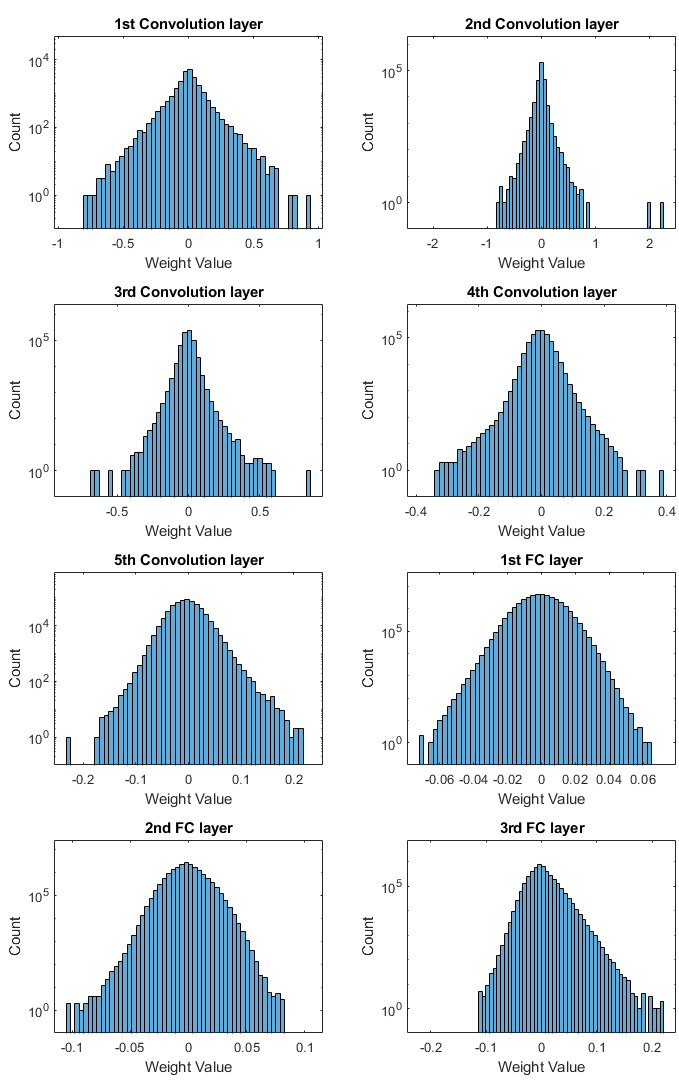
\includegraphics[width=\textwidth]{../Images/Weights-distributions/all-layer-original-weights-distributions.png}
	\decoRule
	\caption[All layer weights distributions]{All layer weights distributions.}
	\label{fig:all-layer-original-weights-distributions}
\end{figure}

Table \ref{tab:pruning-amount-vs-accuracy} shows the weight pruning percentage per layer and all-layer total, with the classification accuracy yielded by each test. Seven tests are depicted, with different configurations each. Tests 1-4 use pruning on all layers, while tests 5-7 use pruning only on the Fully-Connected layers due to their enormous size (see table \ref{tab:AlexNet-Parameters-Memory-Footprint}).

Tests explanation:
\begin{itemize}
	\item \textbf{Test 1:} Low pruning amount on convolution layers, low pruning amount on Fully-Connected layers.
	\item \textbf{Test 2:} Medium pruning amount on convolution layers, low pruning amount on Fully-Connected layers.
	\item \textbf{Test 3:} High pruning amount on convolution layers, low pruning amount on Fully-Connected layers.
	\item \textbf{Test 4:} High pruning amount on convolution layers, high pruning amount on Fully-Connected layers.
	\item \textbf{Test 5:} No pruning on convolution layers, low pruning amount on Fully-Connected layers.
	\item \textbf{Test 6:} No pruning on convolution layers, medium pruning amount on Fully-Connected layers.
	\item \textbf{Test 7:} No pruning on convolution layers, high pruning amount on Fully-Connected layers.
\end{itemize}

\begin{table}[H]
	\caption{All pruning amount configurations tested and their accuracy.}
	\label{tab:pruning-amount-vs-accuracy}
	\centering
	\begin{tabular}{llll llll}
		\toprule
		\textbf{Layer} & \textbf{Test 1} & \textbf{Test 2} & \textbf{Test 3} & \textbf{Test 4} & \textbf{Test 5} & \textbf{Test 6} & \textbf{Test 7}\\
		\midrule
			Conv1 (\%) & 7.15 & 13.66 & 91.3 & 91.3 & 0 & 0 & 0 \\
			Conv2 (\%) & 13.82 & 26.9 & 95.83 & 95.83 & 0 & 0 & 0 \\
			Conv3 (\%) & 13.54 & 26.63 & 98.62 & 98.62 & 0 & 0 & 0 \\
			Conv4 (\%) & 15.32 & 29.99 & 93.14 & 93.14 & 0 & 0 & 0 \\
			Conv5 (\%) & 15.55 & 30.53 & 94.02 & 94.02 & 0 & 0 & 0 \\
			FC1 (\%) & 41.23 & 41.23 & 41.23 & 94.48 & 41.23 & 71.89 & 96.61 \\
			FC2 (\%) & 36.69 & 36.69 & 36.69 & 90.61 & 36.69 & 62.52 & 90.61 \\
			FC3 (\%) & 27.27 & 27.27 & 27.27 & 89.68 & 27.27 & 47.74 & 75.56 \\
			\midrule
			\textbf{Total (\%)} & 37.97	& 38.54 & 41.22 & 93.11 & 37.38 & 64.79 & 89.65 \\
			\midrule
			\textbf{Accuracy (\%)} & 91.74	& 80.8 & 0 & 0 & 90.87 & 71.77 & 15.06 \\
		\bottomrule
	\end{tabular}
\end{table}

From table \ref{tab:pruning-amount-vs-accuracy}, it is evident that increasing the pruning amount leads to lower accuracy. Test 1, which has the lowest pruning amount overall, yielded the best results. Similarly, concerning the tests 5-7, where only the Fully-Connected layers have been pruned, the test with the least amount of pruning, Test 5, resulted in the best accuracy. From the tests 1-4, one could argue that the convolution layers are more prone to error when increasing their pruning amount compared to Fully-Connected layers.

Tests 1 and 5 have identical pruning amount on the Fully-Connected layers; however, test 1 also uses pruning on convolution layers. While test 5 uses less pruning overall, it yields slightly lower accuracy compared to test 1. This could be explained because of the denoising characteristics that the weight pruning provides to the systems. Low and non-important weights could be characterized as noise, originating from the training procedure. Hence, cutting off the "noisy" weights could lead to higher accuracy, which is the case with tests 1 and 5.

Figure \ref{fig:pruning-amount-vs-accuracy} shows the two test groups' classification accuracy to total pruning amount. The first test group, tests 1-4, depicted with blue, is the one that all layers are getting pruned, while the second test group, test 5-7, depicted with red, is the one that only the Fully-Connected layers are getting pruned.

\begin{figure} [H]
	\centering
	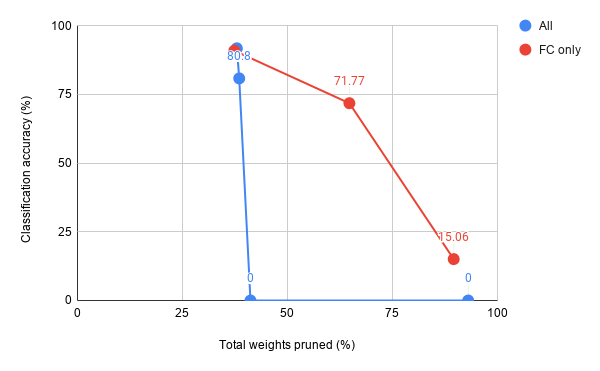
\includegraphics[width=\textwidth]{../Images/Weights-distributions/pruned/pruning-amount-vs-accuracy-chart.png}
	\decoRule
	\caption[Accuracy per pruning amount]{Accuracy per pruning amount.}
	\label{fig:pruning-amount-vs-accuracy}
\end{figure}

It is obvious that pruning only the Fully-Connected layers has much potential and can lead to both high pruning amount and high classification accuracy. However, further investigation has to be conducted for the optimal pruning amount per layer on the whole network.

The effect of weight pruning can be clearly observed in figure \ref{fig:weight-distribution-comparison-pruned-conv1-test3}, which shows the original weight distribution of the first convolution layer (left) compared to the pruned weights distribution (right) of test 3.

\begin{figure} [H]
	\centering
	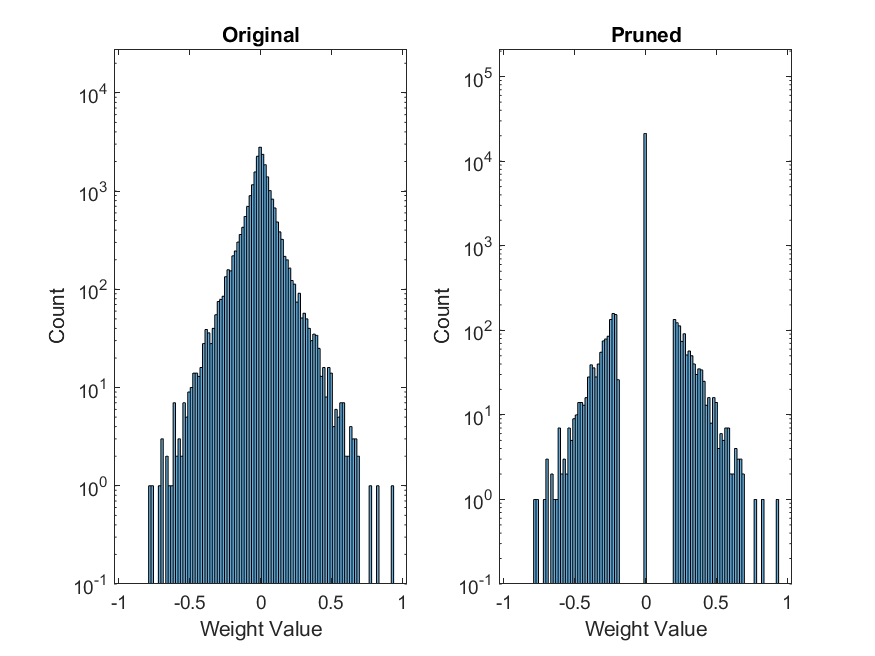
\includegraphics[width=\textwidth]{../Images/Weights-distributions/pruned/41.22/weight-distribution-conv1.png}
	\decoRule
	\caption[Weight distribution comparison of the original and the pruned weights of the first convolution layer of test 3]{Weight distribution comparison of the original and the pruned weights of the first convolution layer  of test 3: A high concentration of zero valued weights can be observed on the pruned weights histogram (right), with a severe absence of near-to-zero valued weights.}
	\label{fig:weight-distribution-comparison-pruned-conv1-test3}
\end{figure}

A high concentration of zeros can be seen on the right histogram, combined with the absence of the near-to-zero valued weights ranging from -0.2 and 0.2. Similar are all layer's weight distributions of test 3, which uses aggressive pruning, creating severe alterations. The weights distributions discontinuity is responsible for the low classification accuracy.

Figures \ref{fig:weight-distribution-comparison-pruned-conv1-test1} and \ref{fig:weight-distribution-comparison-pruned-FC1-test1} demonstrate weight distributions of test 1, which yielded the best classifications overall tests. Those figures are an example of how a pruned distribution should look like to result in relatively high classification accuracy.

Figure \ref{fig:weight-distribution-comparison-pruned-conv1-test1} shows the weight distributions of the first convolution layer with the original and the pruned weights. No discontinuation can be observed on the pruned distribution, and similar to the original concentration of zero-valued weights.

\begin{figure} [H]
	\centering
	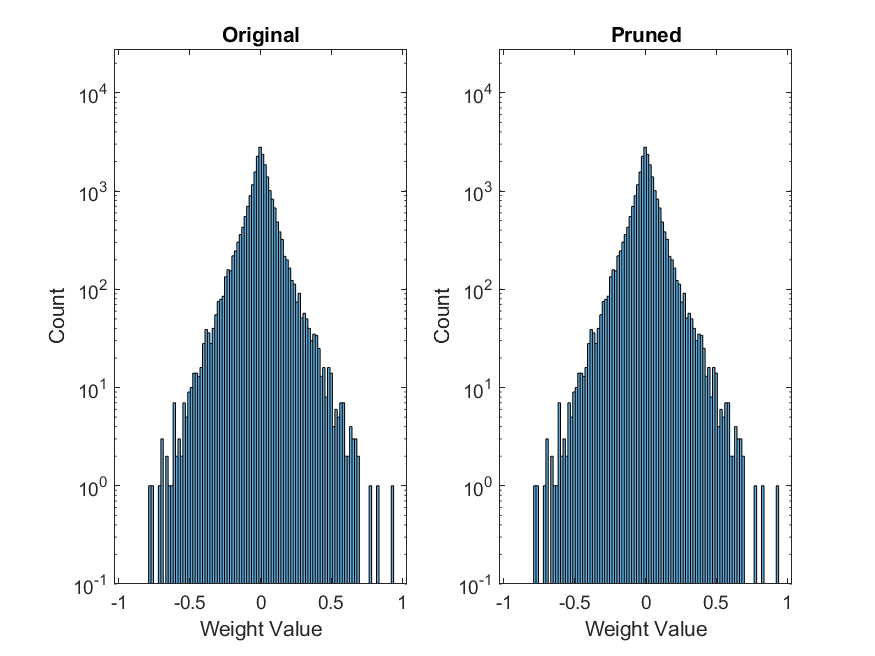
\includegraphics[width=\textwidth]{../Images/Weights-distributions/pruned/37.97/weight-distribution-conv1.png}
	\decoRule
	\caption[Weight distribution comparison of the original and the pruned weights of the first convolution layer of test 1]{Weight distribution comparison of the original and the pruned weights of the first convolution layer of test 1: Similar concentration of zero valued weights can be observed on the pruned histogram (right), with almost no absence of near-to-zero valued weights.}
	\label{fig:weight-distribution-comparison-pruned-conv1-test1}
\end{figure}

Figure \ref{fig:weight-distribution-comparison-pruned-FC1-test1} shows the weight distributions of the first Fully-Connected layer with the original and the pruned weights. Slight discontinuation can be observed on the pruned distribution, with a higher concentration of zero-valued weights. It is vital that the discontinuation is kept really small.

\begin{figure} [H]
	\centering
	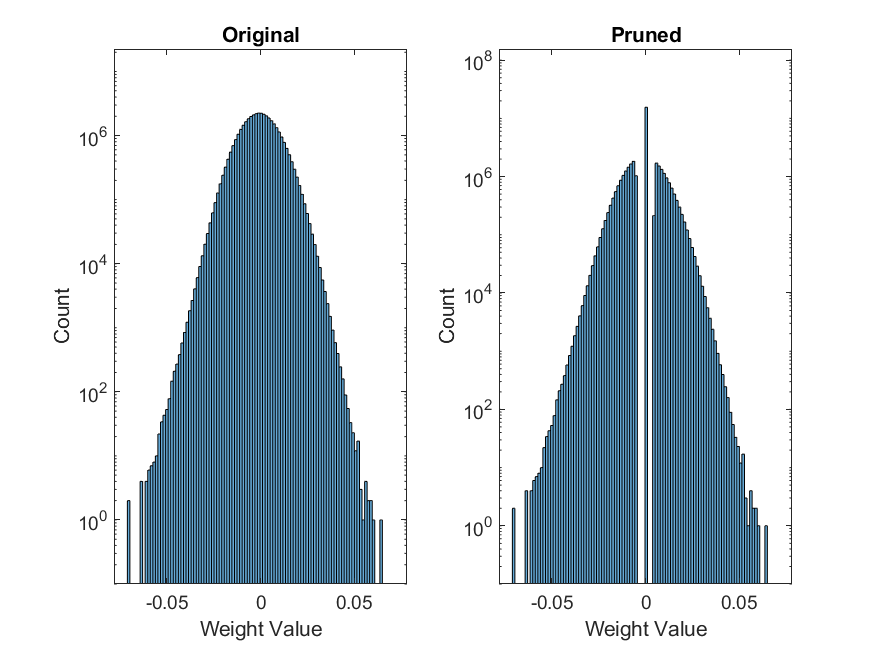
\includegraphics[width=\textwidth]{../Images/Weights-distributions/pruned/37.97/weight-distribution-FC1.png}
	\decoRule
	\caption[Weight distribution comparison of the original and the pruned weights of the first Fully-Connected layer of test 1]{Weight distribution comparison of the original and the pruned weights of the first Fully-Connected layer of test 1: A high concentration of zero valued weights can be observed on the pruned weights histogram (right), with a slight absence of near-to-zero valued weights.}
	\label{fig:weight-distribution-comparison-pruned-FC1-test1}
\end{figure}
